\documentclass{standalone}
\usepackage{helvet}
\usepackage{tikz}
%\usepackage{anyfontsize}
% all other packages and stuff you need for the picture
%

\usetikzlibrary{fit,bayesnet,calc,tikzmark}
\usetikzlibrary{arrows.meta}
\usetikzlibrary{positioning}
\usetikzlibrary{decorations.text}
\usetikzlibrary{decorations.pathmorphing}
\tikzset{squiggle/.style={decorate, decoration={snake,amplitude=.4mm}}}
\usepackage{dsfont}
\usepackage{amsmath}
\usepackage{xcolor}
\definecolor{pop1}{HTML}{1F78b4}
\definecolor{pop2}{HTML}{164C13}
\definecolor{pop3}{HTML}{d95F02}


\usepackage[sfdefault]{FiraSans} %% option 'sfdefault' activates Fira Sans as the default text font
\usepackage[T1]{fontenc}
\renewcommand*\oldstylenums[1]{{\firaoldstyle #1}}



\newcommand{\code}[1]{{\footnotesize\texttt{#1}}}

\newcommand{\NeuralNetwork}[1]{    \begin{tikzpicture}[x=2.5cm,y=1.25cm,transform canvas={scale=#1,shift={+(-1,2.5)}}]
      \tikzstyle{neuron}=[circle,fill=blue!50,minimum size=20pt]
      \fill[fill=teal!5!white] (-0.25,-0.5) rectangle (2.25,-4.5);
      \node[rectangle] at (1,1) {};
      \foreach \name / \y in {1,...,4}
          \node[neuron] (I-\name) at (0,-\y) {};
      \foreach \name / \y in {1,...,3}
          \node[neuron] (H-\name) at (1,-\y-0.5) {};
      \foreach \name / \y in {1,...,4}
          \node[neuron] (O-\name) at (2,-\y) {};
      \foreach \source in {1,...,4}
          \foreach \dest in {1,...,3}
              \draw [-latex] (I-\source) -- (H-\dest);
      \foreach \source in {1,...,3}
          \foreach \dest in {1,...,4}
              \draw [-latex] (H-\source) -- (O-\dest);
    \end{tikzpicture}}
\newcommand{\spiral}[2]{
  \draw[ultra thick,->] ([shift={#1}]-30:#2) arc [radius = #2, start angle = -30, end angle = 90];
  \draw[ultra thick,->] ([shift={#1}]-30:#2) arc [radius = #2, start angle = -30, end angle = 95];

  
      \draw[ultra thick,->] ([shift={#1}]90:#2) arc [radius = #2, start angle = 90, end angle = 210];
      \draw[ultra thick,->] ([shift={#1}]90:#2) arc [radius = #2, start angle = 90, end angle = 205];
      
      \draw[ultra thick,->] ([shift={#1}]210:#2) arc [radius = #2, start angle = 210, end angle = 340];
      \draw[ultra thick,->] ([shift={#1}]210:#2) arc [radius = #2, start angle = 210, end angle = 335];
}
\newcommand{\legend}{
  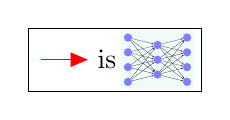
\begin{tikzpicture}
    \node at (0,0) (uses){is};
    \draw[->,red] ([xshift=-0.6cm]uses.west)  -- (uses.west);
    \node at ([xshift=0.4cm]uses.east) {\NeuralNetwork{0.15}};
    \draw[thin] (-1,-0.4) rectangle (1.2,0.4);
  \end{tikzpicture}
  }

\begin{document}\sffamily
\begin{tikzpicture}[line width=0.4mm]
    %% \draw[fill=teal!5!white] (-1.25,1.25) -- (13.25,1.25) -- (13.25,-4) -- (-1.25,-4) -- (-1.25,1.25);
    %% \node at (5.5,1.5) {\textsc{\textbf{Wake}}};

    
%%     \begin{scope}[shift={(0.5,0.5)}]
%%       \node[align=center] at (0,-0.5) (d){
%%         \begin{tabular}{l}
%%           \multicolumn{1}{c}{\textbf{Library}}\\
%%         \small\code{$f_1($x$)=$(+ x 1)}\\
%%         \small\code{$f_2($z$)=$(fold cons}\\
%%         \small\phantom{\code{$f_2($z$)$}}\code{(cons z nil))}\\
%% \small $\cdots\cdots\cdots$
%%                 \end{tabular}};
%%       \node[align=center] at ([yshift = -2cm]d) (t){\textbf{Task}\\
%%         \footnotesize            \code{[7\, 2\, 3]}$\to$\code{[4 3 8]}         \\
%%         \footnotesize    \code{[3\, 8]}$\to$\code{[9 4]}\\
%%         \footnotesize    \code{[4\, 3\, 2]}$\to$\code{[3 4 5]} };

%%       \node at ([xshift = 1.25cm]t.east) (nn){\NeuralNetwork{0.25}};
%%       \node[align = center, text width = 1cm] at ([yshift = 0.7cm,xshift=0cm]nn.north) {\baselineskip=0pt \small Recog. model\par};
%%       \draw [red,-{>[scale=0.2]}] (t.east) -- ([xshift = -0.5cm]nn.west);

%%       \node[draw,rounded corners, align=center, inner sep = 10] at ([xshift = 4.2cm,yshift = 1cm]t.east) (s){Neurally-Guided\\ Enumerative Search};

%%       \draw [red,->] ([xshift = 0.5cm]nn.east) -- ([yshift = -0.25cm]s.west);
%%       \draw [->,rounded corners,] (d.east) -- ([yshift = 2cm]nn.center) -- ([yshift = 0.25cm]s.west);

%%       \node[align=left] at ([xshift=3cm]s.east) (f) {\textbf{Programs for task:}\\
%%         \small    \code{(map $f_1$ (fold $f_2$ nil x))}\\
%%         \small $\cdots\cdots\cdots$};
%%       \draw [->  ] (s.east) -- (f.west);

%%       \draw [->  ,rounded corners] (t.south) -- ([yshift = -0.5cm]t.south) -- ([yshift = -0.5cm] s.south |- t.south) -- (s.south);
%%     \end{scope}
    
    %% \begin{scope}[shift={(9.4,-3.5)},scale=0.6,line width=0.05mm]
    %%   \node[obs,scale=0.7] at (3.5,3) (dx){Library};
    %%   \node[latent,scale=0.7] at ([yshift=-1.7cm,xshift=0cm]dx) (zp){prog};
    %%   \node[obs,scale=0.7] at ([yshift=-1.45cm]zp) (xp) {task};
    %%   \node[latent,scale=0.7] at ([xshift=1.5cm]zp) (zp1){prog};
    %%   \node[obs,scale=0.7] at ([xshift=1.5cm]xp) (xp1) {task};
    %%   \draw [->] (zp1.south) -- (xp1.north);
    %%   \draw [->] (dx.south) -- (zp1.north);
    %%   \draw [->,red] (xp1.east) to[out = 30,in = -30] node(nn){} (zp1.east);
    %%   \node[latent,scale=0.7] at ([xshift=-1.5cm]zp) (zp1){prog};
    %%   \node[obs,scale=0.7] at ([xshift=-1.5cm]xp) (xp1) {task};
    %%   \draw [->] (zp1.south) -- (xp1.north);
    %%   \draw [->] (dx.south) -- (zp1.north);
    %%   \draw [->] (dx.south) -- (zp.north);
    %%   \draw [->] (zp.south) -- (xp.north);
    %%   \draw [->,red] (xp1.east) to[out = 30,in = -30] node(nn){} (zp1.east);
    %%   \draw [->,red] (xp.east) to[out = 30,in = -30] node(nn){} (zp.east);
    %% \end{scope}


    %% \node at (0,-4.75) {\textbf{\textsc{Sleep: Abstraction}}};
    %% \draw[fill=teal!5!white] (-3,-5) -- (3,-5) -- (3,-10) -- (5.5,-10) -- (5.5,-13) -- (-3,-13) -- (-3,-5);
    %% \node at (12,-4.75) {\textbf{\textsc{Sleep: Dreaming}}};
    %% \draw[fill=teal!5!white] (15,-5) -- (9,-5) -- (9,-10) -- (6.5,-10) -- (6.5,-13) -- (15,-13) -- (15,-5);

    %% \begin{scope}[shift={(9.5,-4.5)}]
    %%   \node(dreaming) at (1,-1) {\underline{Fantasies}};
    %%   \node[anchor=center] at ([yshift=-0.5cm]dreaming.south) (d){\textbf{Library}};
    %%   \node at ([yshift=-1.75cm]d.south) (p1){program};
    %%   \draw[squiggle,-> ] (d.south) -- node[sloped,above]{{\small sample}} (p1.north);

    %%   \node(replay) at ([xshift=2cm]dreaming.east) {\underline{Replays}};
    %%   \node[anchor=center,align=center] at ([yshift=-0.5cm]replay.south) (d){\textbf{progs. for task}};
    %%   \node at ([yshift=-1.75cm]d.south) (p1){program};
    %%   \draw[squiggle,-> ] (d.south) -- node[sloped,above]{\small sample} (p1.north);

    %%   \node(p1) at (1.5,-6) {program};      
    %%   \node at ([xshift = 2.0cm]p1.east) (t1){ task};
    %%   \draw [-> ] (p1.east) -- node[above]{\small run} (t1.west);
    %%   \node(n) at ([yshift=-1.2cm,xshift=1.25cm]p1.south) {
    %%     \NeuralNetwork{0.17}};
    %%   \draw [->,red] (t1.south) to[out = -90,in = 0]  ([xshift=0.4cm]n.east);
    %%   \draw [dashed] (p1.south) to[out=-120,in=180] node[above,fill=teal!5!white]{\color{black}Loss} ([xshift=-0.4cm]n.west);


    %%   \node at ($(-0.25,0.5) + (p1.north)!0.5!(t1.north)$) {\underline{Train recognition model}};

    %%   %% \node at ([xshift = 1.5cm]p1.east) (t1){ task};
    %%   %% \draw [-> ] (p1.east) -- node[above]{\small run} (t1.west);
    %%   %% \node(n) at ([yshift=-1.2cm,xshift=0.4cm]p1.south) {
    %%   %%   \NeuralNetwork{0.17}};
    %%   %% \draw [->,red] (t1.south) to[out = -90,in = 0]  ([xshift=0.4cm]n.east);
    %%   %% \draw [dashed] (p1.south) to[out=-120,in=180] node[above,fill=white]{\color{black}Loss} ([xshift=-0.4cm]n.west);

    %%   \begin{scope}[shift={(-3.8,-8)},scale=0.6,line width=0.05mm]
    %%     \node[obs,scale=0.7] at (3.5,3) (dx){Library};
    %%     \node[obs,scale=0.7] at ([yshift=-1.7cm,xshift=0cm]dx) (zp){prog};
    %%     \node[obs,scale=0.7] at ([yshift=-1.45cm]zp) (xp) {task};
    %%     \node[obs,scale=0.7] at ([xshift=1.5cm]zp) (zp1){prog};
    %%     \node[obs,scale=0.7] at ([xshift=1.5cm]xp) (xp1) {task};
    %%     \draw [->] (zp1.south) -- (xp1.north);
    %%     \draw [->] (dx.south) -- (zp1.north);
    %%     \draw [->,red] (xp1.east) to[out = 30,in = -30] node(nn){} (zp1.east);
    %%     \node[obs,scale=0.7] at ([xshift=-1.5cm]zp) (zp1){prog};
    %%     \node[obs,scale=0.7] at ([xshift=-1.5cm]xp) (xp1) {task};
    %%     \draw [->] (zp1.south) -- (xp1.north);
    %%     \draw [->] (dx.south) -- (zp1.north);
    %%     \draw [->] (dx.south) -- (zp.north);
    %%     \draw [->] (zp.south) -- (xp.north);
    %%     \draw [->,red] (xp1.east) to[out = 30,in = -30] node(nn){} (zp1.east);
    %%     \draw [->,red] (xp.east) to[out = 30,in = -30] node(nn){} (zp.east);
    %%   \end{scope}


    %%   \end{scope}

    %% % memory consolidation
    %% \begin{scope}[shift={(-2,-4.5)}]

    %%   %% defined routines for creating fragmented syntax trees
    %%   \newcommand{\syntaxOne}[1]{
    %%     \begin{tikzpicture}[scale=#1,line width=0.35mm]          
    %%       \node(l1) at (0,0) {};
    %%       \node[color=pop3](p1) at (-1,-1) {\texttt{+}};
    %%       \node[color=pop3](n1) at (0.7,-0.9) {\texttt{1}};
    %%       \node(x1) at (0,-1) {\texttt{1}};
    %%       \draw[color=pop3] (l1.south) -- (p1.north);
    %%       \draw[color=pop3] (l1.south) -- (n1.north);
    %%       \draw[color=pop3] (-0.5,-0.45) -- (x1.north);

    %%       \node(t) at (-0.5,0.5) {};
    %%       \draw (l1.south) -- (t.south);
    %%       \node(c) at (-1.5,-0.2) {\texttt{cons}};
    %%       \draw (t.south) -- (c.north);
    %%     \end{tikzpicture}
    %%   }
    %%   \newcommand{\syntaxTo}[1]{
    %%     \begin{tikzpicture}[scale=#1,line width=0.35mm]          
    %%         \node(l1) at (0,0) {};
    %%         \node[color=pop3](p1) at (-1,-1) {\texttt{+}};
    %%         \node[color=pop3](n1) at (0.7,-0.9) {\texttt{1}};
    %%         \draw[color=pop3] (l1.south) -- (p1.north);
    %%         \draw[color=pop3] (l1.south) -- (n1.north);
    %%         \draw[color=pop3] (-0.5,-0.45) -- (0,-1);
    %%         \node(c) at (-0.5,-1.5) {\texttt{car}};
    %%         \node(z) at (0.5,-1.5) {\texttt{z}};
    %%         \draw (0,-1) -- (c.north);
    %%         \draw (0,-1) -- (z.north);
    %%     \end{tikzpicture}
    %%   }

    %%   \node[align=center,anchor=center] at (0.4,-1.2) (f1){\textbf{\footnotesize progs. for task 1}:\\\code{(+ (car z) 1)}};
    %%   \node[align=center] at ([xshift = 1.75cm]f1.east) (f2){\textbf{\footnotesize  progs. for task 2}:\\\code{(cons (+ 1 1))}};
    %%   \node(s1) at ([yshift=-0.5cm]f1.south) {\syntaxOne{0.8}};
    %%   \node(s2) at ([yshift=-0.5cm]f2.south) {\syntaxTo{0.8}};
    %%   \node(c)[align=center,rectangle, rounded corners, draw, minimum width = 4cm, minimum height = 1.5cm, anchor = north] at ($(s1.south)!0.5!(s2.south) + (0,-1)$) {Refactoring Algorithm};
    %%   \draw [-> ] (s1.south) -- (s1.south|-c.north);
    %%   \draw [-> ] (s2.south) -- (s2.south|-c.north);

      
    %%   \node(d) at ([yshift = -1.8cm]c.south) {
    %%     \begin{tikzpicture}[scale=0.9,line width=0.5mm]
    %%       \node[align=center] at (0,0) {\textbf{new Library} w/ \texttt{(+ x 1)}:};
    %%       \begin{scope}[shift={(0.6,-0.5)}]
    %%         \node[pop3](p1) at (-1,-1) {\texttt{+}};
    %%         \node[pop3](n1) at (0.6,-0.9) {\texttt{1}};
    %%         \node[pop3](a) at (0,-1) {\texttt{ }};
    %%         \draw[pop3] (0,0) -- (p1.north);
    %%         \draw[pop3] (0,0) -- (n1.north);
    %%         \draw[pop3] (-0.3,-0.3) -- (a.north);
    %%       \end{scope}
    %%   \end{tikzpicture}};
    %%   \draw [-> ] (c.south) -- (d.north);



    %%   \begin{scope}[shift={(4,-8)},scale=0.6,line width=0.05mm]
    %%     \node[latent,scale=0.7] at (3.5,3) (dx){Library};
    %%     \node[obs,scale=0.7] at ([yshift=-1.7cm,xshift=0cm]dx) (zp){prog};
    %%     \node[obs,scale=0.7] at ([yshift=-1.45cm]zp) (xp) {task};
    %%     \node[obs,scale=0.7] at ([xshift=1.5cm]zp) (zp1){prog};
    %%     \node[obs,scale=0.7] at ([xshift=1.5cm]xp) (xp1) {task};
    %%     \draw [->] (zp1.south) -- (xp1.north);
    %%     \draw [->] (dx.south) -- (zp1.north);
    %%     \node[obs,scale=0.7] at ([xshift=-1.5cm]zp) (zp1){prog};
    %%     \node[obs,scale=0.7] at ([xshift=-1.5cm]xp) (xp1) {task};
    %%     \draw [->] (zp1.south) -- (xp1.north);
    %%     \draw [->] (dx.south) -- (zp1.north);
    %%     \draw [->] (dx.south) -- (zp.north);
    %%     \draw [->] (zp.south) -- (xp.north);
    %%   \end{scope}


    %%   \end{scope}


    
    %% center spiral
    \begin{scope}[shift={(3.25,-7.9)},scale=0.8]    
      %% \spiral{(3.5,1)}{3.5}
      \node[latent,scale=1] at (3.5,3) (dx){Library};
      \node[latent,scale=1] at ([yshift=-2cm,xshift=0cm]dx) (zp){prog};
      \node[obs,scale=1] at ([yshift=-1.45cm]zp) (xp) {task};
      \node[latent,scale=1] at ([xshift=2cm]zp) (zp1){prog};
      \node[obs,scale=1] at ([xshift=2cm]xp) (xp1) {task};
      \draw [->] (zp1.south) -- (xp1.north);
      \draw [->] (dx.south) -- (zp1.north);
      \draw [->,red] (xp1.east) to[out = 30,in = -30] node(nn){} (zp1.east);
      
      \node[latent,scale=1] at ([xshift=-2cm]zp) (zp1){prog};
      \node[obs,scale=1] at ([xshift=-2cm]xp) (xp1) {task};
      \draw [->] (zp1.south) -- (xp1.north);
      \draw [->] (dx.south) -- (zp1.north);
      \draw [->,red] (xp1.east) to[out = 30,in = -30] node(nn){} (zp1.east);


      \draw [->,red] (xp.east) to[out = 30,in = -30] node(nn){} (zp.east);
      \draw [->] (dx.south) -- (zp.north);
      \draw [->] (zp.south) -- (xp.north);

      \node at ([yshift=-0.6cm]xp.south) {\legend};

    \end{scope}    
  \end{tikzpicture}
\end{document}
